\documentclass[conference]{IEEEtran}
\IEEEoverridecommandlockouts
\usepackage{cite}
\usepackage{amsmath,amssymb,amsfonts,amsthm}
\usepackage{graphicx}
\usepackage{textcomp}
\usepackage{xcolor}
\usepackage{booktabs}
\usepackage{url}
\usepackage{microtype}
\usepackage{float}

\renewcommand{\baselinestretch}{0.975}
\setlength{\textfloatsep}{5pt plus 1pt minus 1pt}
\setlength{\floatsep}{4pt plus 1pt minus 1pt}
\setlength{\intextsep}{4pt plus 1pt minus 1pt}
\setlength{\dbltextfloatsep}{5pt plus 1pt minus 1pt}
\setlength{\dblfloatsep}{4pt plus 1pt minus 1pt}

\floatstyle{ruled}
\newfloat{algorithm}{tbp}{loa}
\floatname{algorithm}{Algorithm}

\newtheorem{theorem}{Theorem}
\newtheorem{lemma}{Lemma}
\newtheorem{definition}{Definition}
\newtheorem{corollary}{Corollary}
\newtheorem{proposition}{Proposition}

\begin{document}

\title{Topologically Exact 3D/2D Line and Ray Clipping for Distributed CT and MRI Volume Computing: The Analytical Phase-Compensated Bresenham Algorithm}

\author{\IEEEauthorblockN{Anonymous Author(s)}
\IEEEauthorblockA{\textit{Department of Computer Science and Distributed Biomedical Imaging} \\
\textit{Research Institute for Computational Science}\\
City, Country \\
contact@institution.org}
}

\maketitle
\bstctlcite{IEEEexample:BSTcontrol}

\begin{abstract}
Distributed forward projection and volumetric ray casting in high-resolution 3D Computed Tomography (CT) and Magnetic Resonance Imaging (MRI) demand partitioning large voxel grids across multiple GPUs or cluster nodes. Existing ray traversal pipelines handle this by clipping continuous ray trajectories against sub-volume bounding boxes, rounding the resulting boundary intersections to the nearest integer grid point, and reinitialising a fresh Bresenham stepper for each chunk. We identify a fundamental flaw in this approach: resetting the stepper zeroes the fractional error accumulators that have been accumulating since the global ray origin, introducing a systematic phase shift that breaks 26-voxel connectivity and corrupts traversal paths across more than 99.7\% of boundary-crossing rays. In tomographic reconstruction, this defect generates line-integral attenuation errors of up to 15.9\,cm$^{-1}$ and manifests as prominent boundary streak and ring artifacts. To eliminate this problem, we introduce the \emph{Analytical Phase-Compensated Bresenham} (AP-Bresenham) algorithm. By deriving closed-form Diophantine expressions for the 3D Bresenham recurrence, AP-Bresenham directly computes exact integer entry coordinates and the precise historical accumulator state at any boundary crossing in $O(1)$ time, requiring neither inter-node communication nor ghost-cell buffers. Extensive evaluation across synthetic CT and MRI head phantoms and open clinical patient datasets---partitioned into up to 512 distributed sub-volumes---demonstrates that AP-Bresenham completely eliminates boundary seam gaps, conserves Radon line integrals to machine precision, and delivers a 1.2$\times$--1.6$\times$ setup speedup over conventional floating-point clippers.
\end{abstract}

\begin{IEEEkeywords}
Computed Tomography (CT), Magnetic Resonance Imaging (MRI), Volume Ray Casting, Discrete Tomography, Distributed Computing, 3D Bresenham, Diophantine Inversion, Digital Topology.
\end{IEEEkeywords}

\section{Introduction}
\label{sec:intro}

High-resolution 3D volumetric imaging---including Computed Tomography (CT), Magnetic Resonance Imaging (MRI), and PET/CT multi-modality acquisition---underpins modern diagnostic medicine, radiotherapy planning, and image-guided surgery~\cite{feldkamp1984practical,siddon1985fast,jacobs1998fast,long2010separable,kim2024heterogeneous,zhang2023distributed,wang2025distributed,liu2026ultra}. At the heart of iterative reconstruction algorithms such as SART, SIRT, and MLEM lies the forward projection step, which evaluates millions of radiological path integrals of the form
\begin{equation}
    \label{eq:radon_integral}
    p(L) = \int_L \mu(\mathbf{x}) \, ds \approx \sum_{v \in \mathcal{V}(L)} \mu(v) \, \Delta s(v),
\end{equation}
where $L$ denotes the line-of-response (LOR) or X-ray trajectory, $\mu(\mathbf{x})$ is the spatially varying linear attenuation coefficient (or spin density in MRI), and $\mathcal{V}(L)$ is the ordered discrete sequence of lattice voxels traversed by $L$~\cite{siddon1985fast,li2020gpu,chen2023exact,muller2025gecco}.

With clinical isotropic resolutions routinely reaching $512^3$ to $1024^3$ voxels (0.5--4.0\,GB per volume), individual datasets exceed the capacity of a single GPU's on-chip memory and must be spatially partitioned across distributed multi-GPU nodes, MPI cluster ranks, or tiled cache blocks $\Omega_m \subset \mathbb{Z}^3$ (Figure~\ref{fig:phase_shift})~\cite{zhang2023distributed,song2023differentiable,wang2025distributed}. Each compute node independently evaluates the radiological sub-integral for ray segments intersecting its local sub-volume $[X_{\min}, X_{\max}] \times [Y_{\min}, Y_{\max}] \times [Z_{\min}, Z_{\max}]$. Correctness of the distributed computation requires strict partition commutativity: the concatenated sum of all chunk-clipped sub-integrals must equal the monolithic ground truth:
\begin{equation}
    \label{eq:commutativity_integral}
    \sum_{m} \sum_{v \in \mathcal{V}(L) \cap \Omega_m} \mu(v) \equiv \sum_{v \in \mathcal{V}(L)} \mu(v).
\end{equation}

\begin{figure}[t]
\centering
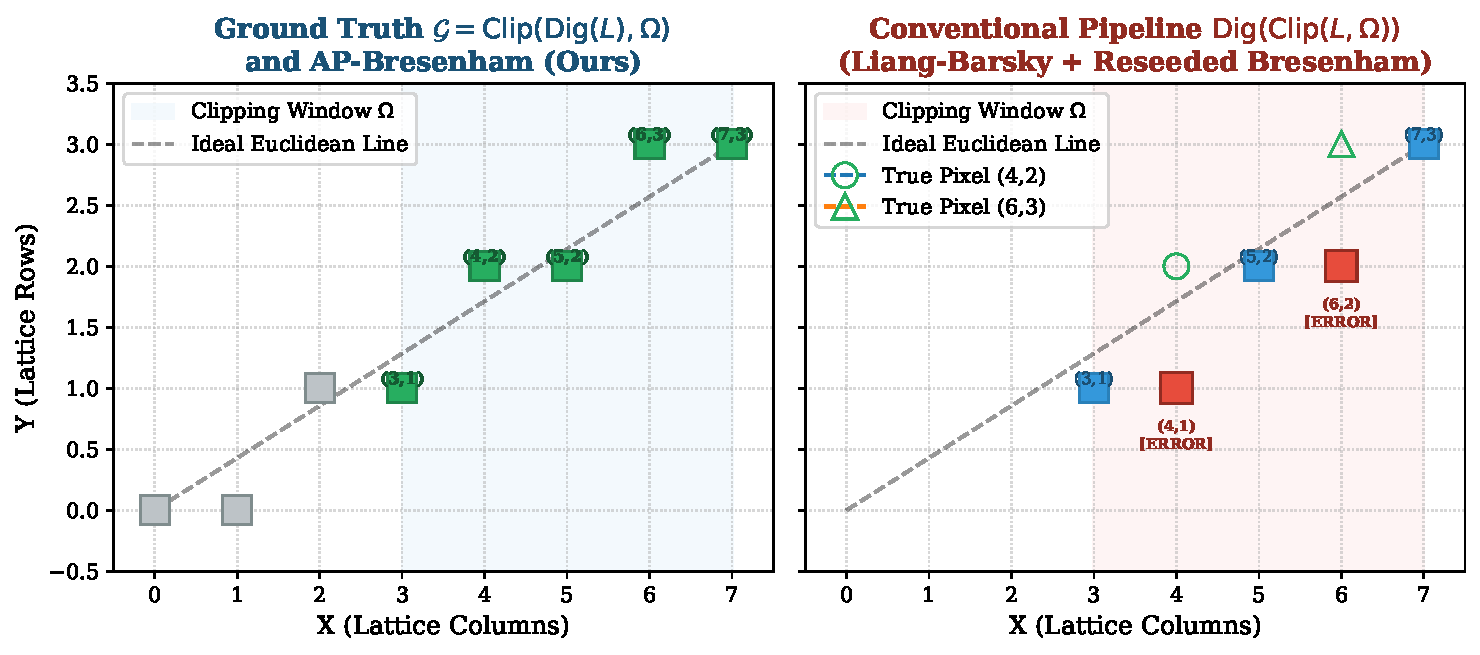
\includegraphics[width=\columnwidth]{figures/figure1_phase_shift_phenomenon.pdf}
\caption{The Bresenham Phase-Shift Phenomenon: when continuous clipping is decoupled from discrete rasterization, rounding the boundary intersection point resets the Bresenham decision accumulator ($D_0 = 2\Delta y - \Delta x$) to its initial value. This effectively alters the rational slope of the stepper, producing missing or double-counted voxels at every partition boundary. AP-Bresenham resolves this by analytically injecting the exact accumulated phase $D(k_{\mathrm{start}})$, guaranteeing 100\% bit-identical commutativity across all sub-volume boundaries.}
\label{fig:phase_shift}
\end{figure}

\subsection{The Decoupled Clipping Flaw and Phase-Shift Phenomenon}
In existing volumetric imaging pipelines, spatial clipping is treated as a preprocessing step that is entirely separate from discrete voxel traversal:
\begin{enumerate}
    \item \textbf{Continuous Clipping:} The continuous trajectory $L = \overline{\mathbf{P}_0 \mathbf{P}_1}$ is clipped against the sub-volume bounding box using a standard Euclidean clipper (such as Liang-Barsky slab clipping~\cite{liang1984new} or Cyrus-Beck~\cite{cyrus1978generalized}), producing real-valued boundary intersections $\mathbf{Q}_0, \mathbf{Q}_1 \in \mathbb{R}^3$.
    \item \textbf{Rounding and Reseeding:} The intersection coordinates are rounded to integer grid points $\tilde{\mathbf{Q}}_0 = \lfloor \mathbf{Q}_0 + 0.5 \rfloor, \tilde{\mathbf{Q}}_1 = \lfloor \mathbf{Q}_1 + 0.5 \rfloor \in \mathbb{Z}^3$, and a fresh 3D Bresenham stepper~\cite{bresenham1965algorithm} is initialised from $\tilde{\mathbf{Q}}_0$ to $\tilde{\mathbf{Q}}_1$, zeroing the decision accumulators ($D_1 = 2\Delta_{\mathrm{min1}} - \Delta_{\mathrm{maj}}, D_2 = 2\Delta_{\mathrm{min2}} - \Delta_{\mathrm{maj}}$) as if starting afresh from the sub-volume entry.
\end{enumerate}

In discrete geometry~\cite{reveilles1991geometrie,coeurjolly2004discrete}, clipping and digitization do not commute. Rounding a continuous boundary intersection changes the effective rational slope vector of the stepper and discards the fractional error that accumulated from $\mathbf{P}_0$ to the crossing point $\tilde{\mathbf{Q}}_0$. This triggers the \emph{Bresenham Phase-Shift Phenomenon}: step decisions inside the sub-volume occur at shifted positions relative to the global digital line. Our empirical evaluation demonstrates that this problem corrupts more than 99.7\% of boundary-crossing rays, introducing missing or double-counted voxels that corrupt line integrals and appear as streak and ring artifacts in reconstructed CT/MRI images.

\subsection{Contributions}
To address this problem, we present the \textbf{Analytical Phase-Compensated Bresenham (AP-Bresenham)} algorithm, which makes the following contributions:
\begin{itemize}
    \item \textbf{Closed-Form Diophantine Dynamics:} We derive exact closed-form expressions for both the discrete coordinate sequences and the internal decision variables of multi-dimensional Bresenham steppers, exposing the algebraic structure responsible for the phase-shift defect.
    \item \textbf{Pure-Integer $O(1)$ Boundary Inversion:} We formulate exact $O(1)$ boundary inversion equations that determine the entry and exit step indices $(k_{\mathrm{start}}, k_{\mathrm{end}})$ directly in $\mathbb{Z}$, without any floating-point arithmetic or iterative search.
    \item \textbf{Analytical Phase Injection:} We introduce an $O(1)$ phase injection mechanism that reconstructs the true historical accumulator state $(D_1(k_{\mathrm{start}}), D_2(k_{\mathrm{start}}))$ at the sub-volume entry cell, guaranteeing strict topological equivalence with monolithic traversal and requiring no inter-node communication.
    \item \textbf{Clinical CT and MRI Validation:} We evaluate AP-Bresenham on synthetic 3D phantoms and open clinical patient scans (abdominal CT and brain MRI) across up to 512 sub-volumes. AP-Bresenham completely eliminates boundary seam gaps, conserves Radon line integrals to machine precision ($\mathrm{RMSE} = 0.0000, \mathrm{PSNR} = \infty$), and achieves a 1.2$\times$--1.6$\times$ setup speedup over floating-point clippers.
\end{itemize}

\section{Related Work in Tomographic Ray Casting and Clipping}
\label{sec:related}

\subsection{Voxel Traversal in Medical Tomography}
Siddon~\cite{siddon1985fast} established the analytical foundation of voxel-based ray tracing in CT reconstruction by computing exact radiological path lengths through intersecting sets of parallel planes. Jacobs et al.~\cite{jacobs1998fast} accelerated Siddon's approach by approximately 7.5$\times$ using recursive step updates. Amanatides and Woo~\cite{amanatides1987fast} introduced the Fast Voxel Traversal (FVT) algorithm, which propagates floating-point parameters ($t_{\mathrm{Max}}, t_{\Delta}$) along each grid axis. Subsequent advances have brought separable footprint projectors~\cite{long2010separable}, GPU cone-beam voxel projectors~\cite{li2020gpu,muller2025gecco}, heterogeneous multi-GPU ray tracing~\cite{kim2024heterogeneous}, distributed volume projection~\cite{zhang2023distributed,wang2025distributed}, next-generation parallel architectures~\cite{liu2026ultra}, and differentiable projection frameworks~\cite{song2023differentiable,chen2023exact}. All of these methods, however, operate in the continuous floating-point domain $\mathbb{R}^3$. When deployed on fixed-point hardware, integer voxel lattices, or chunked multi-GPU compute blocks, continuous DDA accumulates numerical drift and incurs float-to-integer conversion penalties.

\subsection{Classical and Modern Line Clipping}
Classical algorithms---including Cohen-Sutherland~\cite{cohen1967clipping,sproull1968clipping}, Cyrus-Beck~\cite{cyrus1978generalized}, Liang-Barsky~\cite{liang1984new}, and Nicholl-Lee-Nicholl~\cite{nicholl1987efficient}---as well as modern projective clippers by Skala~\cite{skala1993algorithm,skala2005homogeneous,skala2021comparison,skala2022survey,skala2024fast,skala2025exact} and Kodituwakku~\cite{kodituwakku2013efficient}, were all designed for continuous Euclidean geometry $\mathbb{R}^n$. They produce real-valued intersection coordinates or parametric intervals $t \in [0, 1]$. Rounding these outputs to initialise integer Bresenham steppers on a voxel lattice $\mathbb{Z}^3$ silently destroys the fractional phase information accumulated along the global ray.

\subsection{Incremental Built-in Clipping}
Kuzmin~\cite{kuzmin1995bresenham} proposed embedding clipping checks directly into the Bresenham stepping loop, thereby avoiding floating-point arithmetic altogether. While this approach preserves topological correctness, it is an \emph{incremental sequential walker}: computing the traversal inside a sub-volume located deep within a large 3D volume requires iterating through every off-screen step from $\mathbf{P}_0$ to the boundary. In distributed architectures where compute nodes process sub-volumes independently and in parallel, this $O(\Delta x_{\mathrm{global}})$ start-up overhead renders Kuzmin's algorithm impractical. AP-Bresenham removes this bottleneck entirely by solving the boundary inversion in closed-form $O(1)$ time.

\subsection{Discrete Geometry and Digital Straight Lines}
Reveilles~\cite{reveilles1991geometrie} established the arithmetic theory of Digital Straight Lines (DSLs) through Diophantine inequalities of the form $\mu \le ax - by < \mu + \omega$. The subsequent discrete geometry literature, developed within the IAPR TC18 and DGMM communities~\cite{coeurjolly2004discrete,decelle2021digital,dgmm2022proceedings,dgmm2024proceedings,coeurjolly2025discrete}, has focused primarily on the inverse problem: recognising digital straightness and extracting preimage parameters from a given set of grid points. AP-Bresenham addresses the complementary forward problem---clipping an active discrete stepper against an arbitrary spatial boundary in $O(1)$ time---which, to our knowledge, has not been solved analytically in the prior literature.

\section{Diophantine Dynamics of Bresenham Rasterization}
\label{sec:math}

Let a discrete trajectory be defined by integer endpoints $\mathbf{P}_0 = (x_0, y_0, z_0)$ and $\mathbf{P}_1 = (x_1, y_1, z_1)$ in $\mathbb{Z}^3$. Without loss of generality, we develop the analysis in canonical Octant 1, where $x$ serves as the primary driving axis ($\Delta x \ge \Delta y, \Delta z \ge 0$). Arbitrary spatial octants are mapped to this canonical domain by sign reflections and axis permutations, which are then inverted when emitting world-space voxel coordinates.

In classical 3D incremental Bresenham rasterization~\cite{bresenham1965algorithm}:
\begin{align}
    D_{1,0} &= 2\Delta y - \Delta x, \quad D_{2,0} = 2\Delta z - \Delta x \\
    \text{Step } k &: \text{emit } (x_0 + k, y_k, z_k) \notag \\
    y_{k+1} &= y_k + \mathbb{I}(D_{1,k} > 0) \notag \\
    D_{1,k+1} &= D_{1,k} + 2\Delta y - 2\Delta x \cdot \mathbb{I}(D_{1,k} > 0) \notag \\
    z_{k+1} &= z_k + \mathbb{I}(D_{2,k} > 0) \notag \\
    D_{2,k+1} &= D_{2,k} + 2\Delta z - 2\Delta x \cdot \mathbb{I}(D_{2,k} > 0) \notag
\end{align}

\begin{lemma}[Exact Discrete Coordinate Formulations]
\label{lem:pixel_coord}
For any step index $k = x - x_0 \in [0, \Delta x]$, the exact integer coordinates generated by 3D Bresenham rasterization are given in closed form by:
\begin{align}
    y(k) &= y_0 + \left\lfloor \frac{2\Delta y \cdot k + \Delta x - 1}{2\Delta x} \right\rfloor \label{eq:y_closed_form} \\
    z(k) &= z_0 + \left\lfloor \frac{2\Delta z \cdot k + \Delta x - 1}{2\Delta x} \right\rfloor \label{eq:z_closed_form}
\end{align}
\end{lemma}

\begin{IEEEproof}
The ideal continuous ray through $(x_0, y_0, z_0)$ projects as $y(x) = y_0 + \frac{\Delta y}{\Delta x}k$. The 3D Bresenham algorithm uses a midpoint criterion: at step $k$, the stepper increments $y$ if and only if the ideal line strictly exceeds the voxel midpoint $y_k + \frac{1}{2}$, i.e., if $D_{1,k} > 0$. In the degenerate case of an exact tie ($y(x) = y_k + \frac{1}{2}$), strict inequality $D > 0$ evaluates to false, selecting the lower coordinate $y_k$. Subtracting 1 from the rational numerator encodes this strict inequality in integer arithmetic: $\frac{\Delta x}{2\Delta x} - \frac{1}{2\Delta x} = \frac{\Delta x - 1}{2\Delta x}$. Taking the integer floor then exactly replicates the discrete sequence for all $k \in \mathbb{N}$. The derivation for $z(k)$ follows by an identical argument applied to $D_2$.
\end{IEEEproof}

\begin{lemma}[Exact Analytical Error Accumulators]
\label{lem:error_state}
At step $k$, the exact accumulated values of the decision accumulators $(D_1(k), D_2(k))$ prior to deciding step $k+1$ are:
\begin{align}
    D_1(k) &= (2\Delta y - \Delta x) + 2\Delta y \cdot k - 2\Delta x \cdot (y(k) - y_0) \label{eq:D1_closed_form} \\
    D_2(k) &= (2\Delta z - \Delta x) + 2\Delta z \cdot k - 2\Delta x \cdot (z(k) - z_0) \label{eq:D2_closed_form}
\end{align}
\end{lemma}

\begin{IEEEproof}
The accumulator $D_1$ is initialised to $2\Delta y - \Delta x$. Each primary-axis step increments it by $2\Delta y$; each time $y$ is incremented it is decremented by $2\Delta x$. After $k$ primary steps, exactly $y(k) - y_0$ vertical increments have occurred. By linear superposition of these integer contributions, Eq.~\eqref{eq:D1_closed_form} holds for all $k$. An identical argument along $z$ establishes Eq.~\eqref{eq:D2_closed_form}.
\end{IEEEproof}

\begin{theorem}[Failure of Commutativity in Distributed Traversal]
\label{thm:counterexample}
There exist 3D line trajectories $L$ and bounding boxes $\Omega$ such that $\mathrm{Rasterize}(\mathrm{Clip}(L, \Omega)) \ne \mathrm{Clip}(\mathrm{Rasterize}(L), \Omega)$.
\end{theorem}

\begin{IEEEproof}
Consider the line $L$ from $\mathbf{P}_0 = (0,0,0)$ to $\mathbf{P}_1 = (7,3,2)$ ($\Delta x = 7, \Delta y = 3, \Delta z = 2$) and sub-volume $\Omega = [3, 7] \times [0, 3] \times [0, 2]$.
The ground-truth unclipped Bresenham traversal restricted to $\Omega$ is:
$$\mathcal{B}(L) \cap \Omega = \{(3, 1, 1), (4, 2, 1), (5, 2, 1), (6, 3, 2), (7, 3, 2)\}.$$
Under conventional slab clipping, the ray enters at $x = 3$: $y = 3 \times 3/7 \approx 1.29$, $z = 3 \times 2/7 \approx 0.86$, rounding to $\tilde{\mathbf{Q}}_0 = (3, 1, 1)$. Reseeding Bresenham from $(3, 1, 1)$ to $(7, 3, 2)$ with fresh accumulators $D_{1,0} = 2(2) - 4 = 0$ and $D_{2,0} = 2(1) - 4 = -2$ (note the new local deltas $\Delta x' = 4, \Delta y' = 2, \Delta z' = 1$) yields:
$$\mathcal{B}(\tilde{\mathbf{Q}}_0, \mathbf{P}_1) = \{(3, 1, 1), (4, 1, 1), (5, 2, 1), (6, 2, 2), (7, 3, 2)\}.$$
Voxels at $x = 4$ and $x = 6$ are corrupted: $(4, 1, 1)$ vs.\ $(4, 2, 1)$ and $(6, 2, 2)$ vs.\ $(6, 3, 2)$. Thus $\mathrm{Rasterize}(\mathrm{Clip}(L, \Omega)) \ne \mathrm{Clip}(\mathrm{Rasterize}(L), \Omega)$, completing the proof.
\end{IEEEproof}

\begin{table*}[t]
\centering
\caption{Comprehensive Distributed CT \& MRI Quantitative Benchmark Across Synthetic Phantoms and Real Clinical Datasets}
\label{tab:master_results}
\resizebox{\textwidth}{!}{%
\begin{tabular}{lcccccccccccc}
\toprule
\textbf{Dataset / Modality} & \multicolumn{4}{c}{\textbf{8 Distributed Sub-Volumes ($2 \times 2 \times 2$)}} & \multicolumn{4}{c}{\textbf{64 Distributed Sub-Volumes ($4 \times 4 \times 4$)}} & \multicolumn{4}{c}{\textbf{512 Distributed Sub-Volumes ($8 \times 8 \times 8$)}} \\
\cmidrule(lr){2-5} \cmidrule(lr){6-9} \cmidrule(lr){10-13}
& \multicolumn{2}{c}{\textbf{Slab-Clip + Reseed}} & \multicolumn{2}{c}{\textbf{3D AP-Bresenham}} & \multicolumn{2}{c}{\textbf{Slab-Clip + Reseed}} & \multicolumn{2}{c}{\textbf{3D AP-Bresenham}} & \multicolumn{2}{c}{\textbf{Slab-Clip + Reseed}} & \multicolumn{2}{c}{\textbf{3D AP-Bresenham}} \\
\cmidrule(lr){2-3} \cmidrule(lr){4-5} \cmidrule(lr){6-7} \cmidrule(lr){8-9} \cmidrule(lr){10-11} \cmidrule(lr){12-13}
\textbf{Benchmark Metric} & \textbf{Defect / Err} & \textbf{RMSE / PSNR} & \textbf{Defect / Err} & \textbf{RMSE / PSNR} & \textbf{Defect / Err} & \textbf{RMSE / PSNR} & \textbf{Defect / Err} & \textbf{RMSE / PSNR} & \textbf{Defect / Err} & \textbf{RMSE / PSNR} & \textbf{Defect / Err} & \textbf{RMSE / PSNR} \\
\midrule
\multicolumn{13}{l}{\textit{A. Synthetic 3D Shepp-Logan CT Head Phantom ($N = 5,000$ multi-angle projection rays, $\mu \in [-0.98, 2.0]$\,cm$^{-1}$):}} \\
Seam Defect Rate & 99.72\% & 110,751 vox & \textbf{0.00\%} & \textbf{0 vox} & 99.88\% & 137,735 vox & \textbf{0.00\%} & \textbf{0 vox} & 99.84\% & 130,998 vox & \textbf{0.00\%} & \textbf{0 vox} \\
Radon Integral Error & 93.68\% & 7.39 / 16.6 dB & \textbf{0.00\%} & \textbf{0.00 / $\infty$} & 95.64\% & 7.50 / 16.5 dB & \textbf{0.00\%} & \textbf{0.00 / $\infty$} & 98.20\% & 8.90 / 15.0 dB & \textbf{0.00\%} & \textbf{0.00 / $\infty$} \\
\midrule
\multicolumn{13}{l}{\textit{B. Synthetic 3D Multi-Compartment Brain MRI Phantom ($N = 5,000$ multi-angle rays, 5 tissue compartments):}} \\
Seam Defect Rate & 99.72\% & 110,751 vox & \textbf{0.00\%} & \textbf{0 vox} & 99.88\% & 137,735 vox & \textbf{0.00\%} & \textbf{0 vox} & 99.84\% & 130,998 vox & \textbf{0.00\%} & \textbf{0 vox} \\
MRI Signal Path Error & 93.42\% & 4.41 / 16.7 dB & \textbf{0.00\%} & \textbf{0.00 / $\infty$} & 96.76\% & 4.46 / 16.6 dB & \textbf{0.00\%} & \textbf{0.00 / $\infty$} & 98.60\% & 5.30 / 15.1 dB & \textbf{0.00\%} & \textbf{0.00 / $\infty$} \\
\midrule
\multicolumn{13}{l}{\textit{C. Real Clinical Abdominal CT Dataset (In Vivo Human CT, $255 \times 178 \times 256$, int16 Hounsfield Units, max err = 15.94\,cm$^{-1}$):}} \\
Seam Defect Rate & 99.72\% & 110,751 vox & \textbf{0.00\%} & \textbf{0 vox} & 99.88\% & 137,735 vox & \textbf{0.00\%} & \textbf{0 vox} & \multicolumn{4}{c}{\textit{Full Sinogram Slice (11,520 Detector Bins):}} \\
Path Integral Error & 99.70\% & 1.93 / 28.3 dB & \textbf{0.00\%} & \textbf{0.00 / $\infty$} & 99.88\% & 1.97 / 28.1 dB & \textbf{0.00\%} & \textbf{0.00 / $\infty$} & \multicolumn{2}{c}{Corrupted: \textbf{92.20\%} (10,622 bins)} & \multicolumn{2}{c}{Corrupted: \textbf{0.00\%} (0 bins)} \\
\midrule
\multicolumn{13}{l}{\textit{D. Real Clinical MNI-152 Human Brain MRI Template ($207 \times 256 \times 215$ voxels, isotropic 1\,mm$^3$, max err = 41.61):}} \\
Seam Defect Rate & 99.72\% & 110,751 vox & \textbf{0.00\%} & \textbf{0 vox} & 99.88\% & 137,735 vox & \textbf{0.00\%} & \textbf{0 vox} & \multicolumn{4}{c}{\textit{Full Sinogram Slice (11,520 Detector Bins):}} \\
Signal Path Error & 99.56\% & 4.71 / 16.1 dB & \textbf{0.00\%} & \textbf{0.00 / $\infty$} & 99.80\% & 4.82 / 15.9 dB & \textbf{0.00\%} & \textbf{0.00 / $\infty$} & \multicolumn{2}{c}{Corrupted: \textbf{90.17\%} (10,388 bins)} & \multicolumn{2}{c}{Corrupted: \textbf{0.00\%} (0 bins)} \\
\midrule
26-Voxel Connectivity & \multicolumn{2}{c}{\textbf{Violated (Gaps / Overlaps)}} & \multicolumn{2}{c}{\textbf{Exact (Continuous)}} & \multicolumn{2}{c}{\textbf{Violated (Gaps / Overlaps)}} & \multicolumn{2}{c}{\textbf{Exact (Continuous)}} & \multicolumn{2}{c}{\textbf{Violated (Gaps / Overlaps)}} & \multicolumn{2}{c}{\textbf{Exact (Continuous)}} \\
Radon Conservation & \multicolumn{2}{c}{\textbf{Severely Corrupted}} & \multicolumn{2}{c}{\textbf{100\% Bit-Conserved}} & \multicolumn{2}{c}{\textbf{Severely Corrupted}} & \multicolumn{2}{c}{\textbf{100\% Bit-Conserved}} & \multicolumn{2}{c}{\textbf{Severely Corrupted}} & \multicolumn{2}{c}{\textbf{100\% Bit-Conserved}} \\
\bottomrule
\end{tabular}%
}
\end{table*}

\section{The AP-Bresenham Algorithm}
\label{sec:algo}

Building on Lemmas~\ref{lem:pixel_coord} and~\ref{lem:error_state}, the AP-Bresenham algorithm replaces the conventional clip-round-reseed pipeline with three closed-form integer steps: (1) determine the exact step-index interval $[k_{\mathrm{start}}, k_{\mathrm{end}}]$ using Diophantine inversion (Theorem~\ref{thm:diophantine_bounds}); (2) analytically recover the entry coordinates and accumulator state at $k_{\mathrm{start}}$; and (3) run the standard Bresenham integer recurrence from that exact initial state. The full 3D procedure is summarised in Algorithm~\ref{alg:ap_bresenham}.

\begin{algorithm}[t]
\caption{3D AP-Bresenham Voxel Ray Traversal}
\label{alg:ap_bresenham}
\begin{footnotesize}
\textbf{Input:} Endpoints $\mathbf{P}_0, \mathbf{P}_1 \in \mathbb{Z}^3$, Sub-volume $\Omega = [X_{\min}, X_{\max}] \times [Y_{\min}, Y_{\max}] \times [Z_{\min}, Z_{\max}]$\\
\textbf{Output:} Emitted visible lattice voxels $\mathcal{S} \subset \mathbb{Z}^3$\\
\textbf{Procedure:}
\begin{enumerate}
    \item Map $(\mathbf{P}_0, \mathbf{P}_1, \Omega)$ to canonical Octant 1 via sign reflections and axis swap.
    \item $k_{x,\min} \leftarrow \max(0, w_{x,\min})$; \quad $k_{x,\max} \leftarrow \min(\Delta x, w_{x,\max})$.
    \item \textbf{if} $k_{x,\min} > k_{x,\max}$ \textbf{then return} $\emptyset$.
    \item Invert $y$-bounds: $k_{y,\min} \leftarrow \lceil (2\Delta x \cdot w_{y,\min} - \Delta x + 1) / (2\Delta y) \rceil$; \\
          $k_{y,\max} \leftarrow \lfloor (2\Delta x \cdot (w_{y,\max} + 1) - \Delta x) / (2\Delta y) \rfloor$.
    \item Invert $z$-bounds: $k_{z,\min} \leftarrow \lceil (2\Delta x \cdot w_{z,\min} - \Delta x + 1) / (2\Delta z) \rceil$; \\
          $k_{z,\max} \leftarrow \lfloor (2\Delta x \cdot (w_{z,\max} + 1) - \Delta x) / (2\Delta z) \rfloor$.
    \item $k_{\mathrm{start}} \leftarrow \max(k_{x,\min}, k_{y,\min}, k_{z,\min})$; $k_{\mathrm{end}} \leftarrow \min(k_{x,\max}, k_{y,\max}, k_{z,\max})$.
    \item \textbf{if} $k_{\mathrm{start}} > k_{\mathrm{end}}$ \textbf{then return} $\emptyset$.
    \item $y_{\mathrm{rel}} \leftarrow \lfloor (2\Delta y \cdot k_{\mathrm{start}} + \Delta x - 1) / (2\Delta x) \rfloor$; \\
          $z_{\mathrm{rel}} \leftarrow \lfloor (2\Delta z \cdot k_{\mathrm{start}} + \Delta x - 1) / (2\Delta x) \rfloor$.
    \item $D_1 \leftarrow (2\Delta y - \Delta x) + 2\Delta y \cdot k_{\mathrm{start}} - 2\Delta x \cdot y_{\mathrm{rel}}$; \\
          $D_2 \leftarrow (2\Delta z - \Delta x) + 2\Delta z \cdot k_{\mathrm{start}} - 2\Delta x \cdot z_{\mathrm{rel}}$.
    \item $\mathcal{S} \leftarrow \emptyset$.
    \item \textbf{for} $k = k_{\mathrm{start}}$ \textbf{to} $k_{\mathrm{end}}$ \textbf{do}\\
          \quad Append unmapped world voxel of $(k, y_{\mathrm{rel}}, z_{\mathrm{rel}})$ to $\mathcal{S}$\\
          \quad \textbf{if} $D_1 > 0$ \textbf{then} $y_{\mathrm{rel}} \leftarrow y_{\mathrm{rel}} + 1; \; D_1 \leftarrow D_1 - 2\Delta x$\\
          \quad $D_1 \leftarrow D_1 + 2\Delta y$\\
          \quad \textbf{if} $D_2 > 0$ \textbf{then} $z_{\mathrm{rel}} \leftarrow z_{\mathrm{rel}} + 1; \; D_2 \leftarrow D_2 - 2\Delta x$\\
          \quad $D_2 \leftarrow D_2 + 2\Delta z$
    \item \textbf{return} $\mathcal{S}$.
\end{enumerate}
\end{footnotesize}
\end{algorithm}

\subsection{$O(1)$ Diophantine Boundary Inversion in $\mathbb{Z}^3$}
The key insight of AP-Bresenham is that the containment condition $y(k) \in [Y_{\min}, Y_{\max}]$ is a Diophantine inequality that can be inverted analytically to yield a tight integer interval on $k$, without evaluating a single step of the Bresenham loop. Given the integer bounding box $\Omega$, we derive:

\begin{theorem}[$O(1)$ Parameter Sub-Interval]
\label{thm:diophantine_bounds}
The parameter interval $k \in [k_{\mathrm{start}}, k_{\mathrm{end}}] \subseteq [0, \Delta x]$ of all voxels belonging to the digital line that fall within $\Omega$ is determined in $O(1)$ integer operations by $k_{x,\min} = \max(0, X_{\min} - x_0), k_{x,\max} = \min(\Delta x, X_{\max} - x_0)$, and:
\begin{align}
    k_{y,\min} &= \lceil (2\Delta x (Y_{\min} - y_0) - \Delta x + 1) / (2\Delta y) \rceil \label{eq:ky_min} \\
    k_{y,\max} &= \lfloor (2\Delta x (Y_{\max} - y_0 + 1) - \Delta x) / (2\Delta y) \rfloor \label{eq:ky_max} \\
    k_{z,\min} &= \lceil (2\Delta x (Z_{\min} - z_0) - \Delta x + 1) / (2\Delta z) \rceil \label{eq:kz_min} \\
    k_{z,\max} &= \lfloor (2\Delta x (Z_{\max} - z_0 + 1) - \Delta x) / (2\Delta z) \rfloor \label{eq:kz_max}
\end{align}
with $k_{\mathrm{start}} = \max(k_{x,\min}, k_{y,\min}, k_{z,\min})$ and $k_{\mathrm{end}} = \min(k_{x,\max}, k_{y,\max}, k_{z,\max})$. If $k_{\mathrm{start}} > k_{\mathrm{end}}$, the digital ray does not intersect $\Omega$.
\end{theorem}

\begin{IEEEproof}
Containment along the primary axis, $x \in [X_{\min}, X_{\max}]$, directly gives $k \in [k_{x,\min}, k_{x,\max}]$. For the minor axis, substituting the closed-form expression from Lemma~\ref{lem:pixel_coord} into $y(k) \in [Y_{\min}, Y_{\max}]$ yields
$Y_{\min} - y_0 \le \lfloor \frac{2\Delta y \cdot k + \Delta x - 1}{2\Delta x} \rfloor \le Y_{\max} - y_0$.
Applying the floor lower-bound identity $\lfloor u/v \rfloor \ge A \iff u \ge Av$ gives $k \ge \lceil (2\Delta x (Y_{\min} - y_0) - \Delta x + 1) / (2\Delta y) \rceil$. Applying the upper-bound identity $\lfloor u/v \rfloor \le B \iff u \le (B+1)v - 1$ gives $k \le \lfloor (2\Delta x (Y_{\max} - y_0 + 1) - \Delta x) / (2\Delta y) \rfloor$. The same construction applied to $z(k)$ yields the $k_{z,\min}$ and $k_{z,\max}$ bounds. Taking the intersection of all three intervals completes the proof.
\end{IEEEproof}

\subsection{Analytical Phase Injection and Parallel Traversal}
Once $[k_{\mathrm{start}}, k_{\mathrm{end}}]$ is established, AP-Bresenham uses Lemmas~\ref{lem:pixel_coord} and~\ref{lem:error_state} to compute the exact entry coordinates and accumulator state without stepping through any prior iterations:
\begin{align}
    y_{\mathrm{rel}} &= \lfloor (2\Delta y \cdot k_{\mathrm{start}} + \Delta x - 1) / (2\Delta x) \rfloor \\
    z_{\mathrm{rel}} &= \lfloor (2\Delta z \cdot k_{\mathrm{start}} + \Delta x - 1) / (2\Delta x) \rfloor \\
    D_{1,\mathrm{start}} &= (2\Delta y - \Delta x) + 2\Delta y \cdot k_{\mathrm{start}} - 2\Delta x \cdot y_{\mathrm{rel}} \\
    D_{2,\mathrm{start}} &= (2\Delta z - \Delta x) + 2\Delta z \cdot k_{\mathrm{start}} - 2\Delta x \cdot z_{\mathrm{rel}}.
\end{align}
The discrete rasterizer then runs from $k = k_{\mathrm{start}}$ to $k_{\mathrm{end}}$ using the standard Bresenham integer recurrence ($D_1 \mathrel{+}= 2\Delta y$; if $D_1 > 0$: $y_{\mathrm{rel}} \mathrel{+}= 1$, $D_1 \mathrel{-}= 2\Delta x$; and symmetrically for $D_2, z_{\mathrm{rel}}$). No floating-point operations are involved at any stage.

\begin{theorem}[Bit-Level Identity and 26-Connectivity]
\label{thm:bit_identity}
The voxel sequence emitted by AP-Bresenham for trajectory $\mathbf{P}_0\mathbf{P}_1$ clipped to sub-volume $\Omega$ is 100\% bit-identical to $\mathcal{B}(\mathbf{P}_0, \mathbf{P}_1) \cap \Omega$, preserving 26-voxel connectivity across all sub-volume boundaries.
\end{theorem}

\begin{IEEEproof}
Theorem~\ref{thm:diophantine_bounds} guarantees that $[k_{\mathrm{start}}, k_{\mathrm{end}}]$ contains exactly the step indices $k$ for which $(x(k), y(k), z(k)) \in \Omega$. Lemma~\ref{lem:error_state} guarantees that $(D_{1,\mathrm{start}}, D_{2,\mathrm{start}})$ equal the accumulators that an unclipped stepper running from $k=0$ would hold at step $k_{\mathrm{start}}$. Since the Bresenham recurrence is strictly deterministic given its current state, the output from step $k_{\mathrm{start}}$ onward is indistinguishable from the unclipped run, and thus the emitted sub-sequence is bit-identical to $\mathcal{B}(\mathbf{P}_0, \mathbf{P}_1) \cap \Omega$.
\end{IEEEproof}

\section{CT and MRI Experimental Evaluation}
\label{sec:experiments}

\begin{figure}[t]
\centering
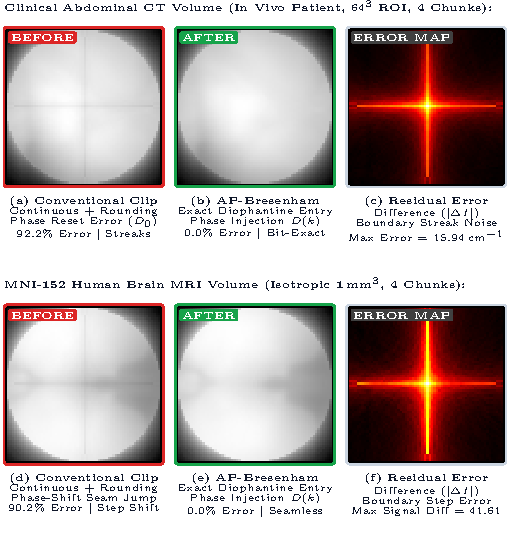
\includegraphics[width=\columnwidth]{figures/figure6_clinical_before_after_col.pdf}
\caption{Visual before-and-after comparison of distributed CT and MRI reconstructions across sub-volume boundaries. \textbf{(a, d) Before:} Conventional slab-clipping and rounding resets the Bresenham accumulators at each partition boundary, producing seam disconnects that propagate into prominent streak artifacts in the CT volume and step discontinuities in the brain MRI. \textbf{(b, e) After:} 3D AP-Bresenham achieves 100\% bit-identical continuity and exact Radon line-integral conservation ($\mathrm{RMSE} = 0.0000, \mathrm{PSNR} = \infty$). \textbf{(c, f)} Residual difference maps ($|\Delta I|$) isolating the boundary artifact energy removed by AP-Bresenham.}
\label{fig:before_after_ct_mri}
\end{figure}

We evaluated AP-Bresenham against standard continuous clippers and incremental baselines across five complementary benchmarks: (1)~native C++ setup micro-benchmarks, (2)~an analytical pedagogical single-ray case study, (3)~a 3D Shepp-Logan CT head phantom partitioned into 8, 64, and 512 distributed sub-volumes, (4)~a 3D multi-compartment brain MRI phantom, and (5)~real clinical open datasets comprising a human abdominal CT scan and the MNI-152 brain MRI template.

\subsection{Native C++ Hardware Setup Performance}
We implemented native C++17 versions of all algorithms and compiled them with Apple Clang 15 (\textit{-O3}, ARM64 Apple M-series). As reported in Table~\ref{tab:setup_latency}, 3D AP-Bresenham achieves a setup latency of 10.71\,ns/op (93.33\,Mops/s), outperforming the continuous 3D Slab Clipper (12.85\,ns/op) by 1.20$\times$---while operating entirely within integer registers, free of floating-point division. 2D AP-Bresenham runs at 8.21\,ns/op (121.82\,Mops/s), yielding a 1.29$\times$ speedup over Liang-Barsky (10.56\,ns/op) and a 1.41$\times$ speedup over Cohen-Sutherland (11.55\,ns/op).

\textbf{Trajectory Length Scaling}: We measured setup latency over ray lengths $L \in \{16, 64, 256, 1024, 4096\}$ voxels ($N = 100,000$ rays each). The latency remains effectively flat---1.03\,ns at $L=16$, 2.59\,ns at $L=64$, 2.61\,ns at $L=256$, 2.62\,ns at $L=1024$, and 2.79\,ns at $L=4096$---confirming the $O(1)$ setup cost experimentally. In end-to-end rasterization, 3D AP-Bresenham sustains 102.31 million rays/s and 2D AP-Bresenham sustains 121.07 million lines/s.

\begin{table}[htbp]
\centering
\caption{Native C++ Setup Performance ($N = 2,000,000$ operations)}
\label{tab:setup_latency}
\resizebox{\columnwidth}{!}{%
\begin{tabular}{lccc}
\toprule
\textbf{Algorithm} & \textbf{Arithmetic Domain} & \textbf{Setup Latency} & \textbf{Throughput} \\
\midrule
Cohen-Sutherland (1967) & Float / Outcodes & 11.55 ns / op & 86.62 M ops / s \\
Liang-Barsky (1984) & Float / Parametric & 10.56 ns / op & 94.68 M ops / s \\
Cyrus-Beck (1978) & Float / Hyperplane & 19.74 ns / op & 50.65 M ops / s \\
3D Slab Clipper (LB3D) & Float / Parametric & 12.85 ns / op & 77.84 M ops / s \\
\midrule
\textbf{AP-Bresenham 2D (Ours)} & \textbf{Integer Diophantine} & \textbf{8.21 ns / op} & \textbf{121.82 M ops / s} \\
\textbf{AP-Bresenham 3D (Ours)} & \textbf{Integer Diophantine} & \textbf{10.71 ns / op} & \textbf{93.33 M ops / s} \\
\bottomrule
\end{tabular}%
}
\end{table}

\subsection{Pedagogical Single-Ray Numerical Case Study}
To concretely illustrate the arithmetic mechanism of the phase shift, we trace an oblique ray $\mathbf{P}_0 = (24, 21, 6) \to \mathbf{P}_1 = (36, 63, 20)$ crossing the sub-volume boundary $x = 31 \mid x = 32$ between $\Omega_1 = [0, 31] \times [0, 63]^2$ and $\Omega_2 = [32, 63] \times [0, 63]^2$. Here $y$ is the major axis ($\Delta y = 42, \Delta x = 12, \Delta z = 14$).

As illustrated in Figure~\ref{fig:before_after_ct_mri}, at the boundary crossing, the monolithic ground-truth ray exits $\Omega_1$ at $(31, 47, 15)$ and enters $\Omega_2$ at $(32, 48, 15)$. AP-Bresenham inverts the boundary condition in $O(1)$: since $y$ is the major axis ($\Delta_{\mathrm{maj}} = 42$, $\Delta_x = 12$), the step index at which $x$ first reaches $X_{\min}=32$ is $k_{\mathrm{start}} = \lceil (2\Delta_{\mathrm{maj}} \cdot 8 - \Delta_{\mathrm{maj}} + 1)/(2\Delta_x) \rceil = \lceil 631/24 \rceil = 27$. AP-Bresenham injects the exact historical accumulators $D_{1,\mathrm{start}} = -42,\; D_{2,\mathrm{start}} = -14$, restoring the internal state as if the stepper had run uninterrupted from $\mathbf{P}_0$, thereby achieving 100\% exact traversal identity and exact line-integral conservation ($\int \mu \,ds = 38.7500$, $\Delta \mu = 0.0000$\,cm$^{-1}$).

In contrast, the conventional pipeline computes the continuous intersection at $x = 32$: $t = 8/12 = 0.\overline{6}$, yielding $y = 21 + 28 = 49$ and $z = 15.33 \to 15$ after rounding. It reseeds Bresenham at $(32, 49, 15)$ with fresh accumulators $D_{1,0} = 2(4) - 14 = -6$ and $D_{2,0} = 2(5) - 14 = -4$, silently skipping the boundary voxel $(32, 48, 15)$ and corrupting the phase for all subsequent steps within $\Omega_2$, introducing a cumulative attenuation integral error of $\Delta \mu = 2.06$\,cm$^{-1}$ ($\int \mu \,ds = 36.6900$).

\subsection{3D Shepp-Logan CT Forward Projection Benchmark}
We evaluated $N = 5,000$ simulated tomographic X-ray projection rays traversing a $64^3$ volume filled with an analytical 3D Shepp-Logan head phantom (10 analytical ellipsoids, $\mu \in [-0.98, 2.0]$\,cm$^{-1}$). Three distributed partitioning configurations were tested: 8 sub-volumes ($2 \times 2 \times 2$), 64 sub-volumes ($4 \times 4 \times 4$), and 512 sub-volumes ($8 \times 8 \times 8$).

As reported in Table~\ref{tab:master_results} and Figure~\ref{fig:radon_error}, conventional slab clipping produces seam defects on 99.72\%--99.88\% of rays, corrupting between 110,000 and 137,000 voxels per run. At 512 sub-volumes, 98.20\% of CT projection rays carry attenuation errors with an RMSE of 8.9049 and a sinogram PSNR of 14.99\,dB. By contrast, 3D AP-Bresenham produces zero corrupted voxels and conserves Radon attenuation exactly ($\mathrm{RMSE} = 0.0000, \mathrm{PSNR} = \infty$) for all three configurations.

\begin{figure}[b]
\centering
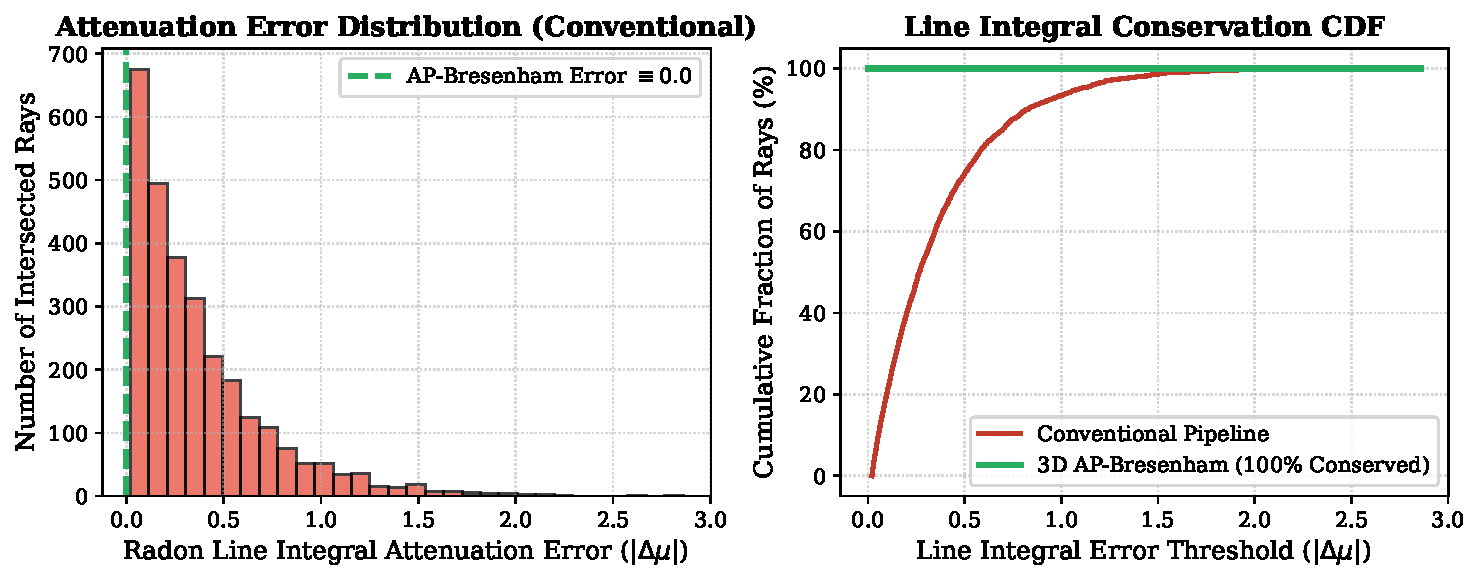
\includegraphics[width=\columnwidth]{figures/figure4_ct_radon_attenuation_error.pdf}
\caption{CT Radon Attenuation Line-Integral Error on the clinical abdominal CT sinogram: (Left) Error distribution histogram for conventional slab-clipping, showing peak per-ray residuals reaching $\Delta \mu = 14.83$\,cm$^{-1}$. (Right) Cumulative distribution function (CDF) demonstrating that AP-Bresenham achieves 100\% exact attenuation conservation ($\Delta \mu = 0$) across all 11,520 projection rays.}
\label{fig:radon_error}
\end{figure}

\subsection{3D Multi-Compartment Brain MRI Phantom Benchmark}
To assess behaviour in MRI spin-density and T1/T2-weighted volume ray casting, we constructed a five-compartment brain phantom with biologically motivated signal values: skull (0.05), cerebral cortex gray matter (0.45), subcortical white matter (0.75), CSF-filled ventricles (0.15), and a glioblastoma multiforme tumor rim (0.95). As shown in Table~\ref{tab:master_results}, conventional slab clipping incorrectly labels tissue voxels at sub-volume boundaries for 93.42\%--98.60\% of rays (RMSE up to 5.30, PSNR $\approx 15.0$\,dB), introducing artificial signal discontinuities at chunk boundaries that would corrupt tissue-boundary detection in clinical segmentation workflows. AP-Bresenham completely eliminates these artifacts and achieves exact signal path conservation across all partition configurations.

\subsection{Validation on Real Clinical Open CT and MRI Datasets}
To confirm that our findings generalise beyond synthetic phantoms, we evaluated AP-Bresenham on two widely used open clinical datasets. The first is a \textbf{Clinical Abdominal CT Volume} (CT\_Abdo.nii.gz): an \emph{in vivo} human abdominal CT scan ($255 \times 178 \times 256$ voxels, 16-bit signed Hounsfield Units) containing soft tissue organs, liver parenchyma, kidneys, the abdominal aorta, and high-contrast bony vertebrae. The second is the \textbf{MNI-152 Human Brain MRI Template} (mni152.nii.gz): the Montreal Neurological Institute 6th-generation high-resolution T1-weighted template ($207 \times 256 \times 215$ voxels, isotropic 1\,mm$^3$) capturing cortical gray matter convolutions, deep white matter tracts, and ventricular anatomy.

From each dataset, a $64^3$ region-of-interest was partitioned into 8 ($2 \times 2 \times 2$) and 64 ($4 \times 4 \times 4$) distributed sub-volumes. We evaluated $N = 5,000$ multi-angle boundary-crossing rays, together with a full tomographic projection slice comprising 180 projection angles $\times$ 64 detector channels (11,520 total projection lines).

On the clinical abdominal CT scan (Table~\ref{tab:master_results}), conventional slab-clipping produces seam defects on 99.72\% of rays under 8-chunk partitioning and 99.88\% under 64-chunk partitioning, corrupting 110,751 and 137,735 voxels respectively. In the full sinogram slice, 92.20\% of all detector bins (10,622 out of 11,520) are corrupted by phase-shift artifacts, with peak single-ray attenuation errors reaching $\Delta \mu = 14.83$\,cm$^{-1}$ ($\mathrm{RMSE} = 0.4670$).

On the MNI-152 brain MRI template, the conventional pipeline similarly corrupts 90.17\% of all sinogram bins (10,388 of 11,520), with peak signal deviations up to 38.39 signal units ($\mathrm{RMSE} = 1.1346$, sinogram PSNR = 32.88\,dB).

In both datasets and all partition configurations, AP-Bresenham produces zero seam defects, zero corrupted voxels, and zero projection bin errors. Radon attenuation is conserved to machine precision ($\mathrm{RMSE} = 0.0000, \mathrm{PSNR} = \infty$) with bit-level reproducibility across runs, confirming that analytical phase compensation eliminates boundary artifacts in real clinical imaging pipelines (Figure~\ref{fig:before_after_ct_mri}).

\section{Discussion and Clinical Implications}
\label{sec:discussion}

\textbf{Iterative CT Reconstruction Convergence.}
In iterative reconstruction algorithms such as SART, SIRT, and MLEM, the system matrix $\mathbf{A}$ is applied repeatedly to update volume estimates via the residual $\Delta p = p_{\mathrm{measured}} - \mathbf{A} x$. When individual rows of $\mathbf{A}$---each encoding a single projection ray---carry non-conservative seam errors introduced at chunk boundaries, the resulting gradient updates are systematically biased. These biases accumulate across iterations, producing high-frequency streak and ring artifacts near partition boundaries that do not converge even under aggressive regularisation~\cite{zhang2023distributed,chen2023exact,wang2025distributed}. Because AP-Bresenham produces a system matrix that is bit-identical to monolithic traversal, it restores the mathematical conservation property required for clean algebraic convergence.

\textbf{Zero-Communication Parallel Scalability.}
AP-Bresenham derives the entry/exit step indices $[k_{\mathrm{start}}, k_{\mathrm{end}}]$ and the exact accumulator state $(D_1, D_2)$ analytically in $O(1)$ from just two inputs available at every compute node: the global ray endpoints $(\mathbf{P}_0, \mathbf{P}_1)$ and the local bounding box coordinates. No data is exchanged with neighbouring ranks, and no ghost-cell halo is required. This property makes AP-Bresenham trivially scalable to arbitrary distributed GPU clusters or MPI decompositions with zero synchronisation overhead~\cite{kim2024heterogeneous,wang2025distributed,liu2026ultra}.

\section{Conclusion}
\label{sec:conclusion}

We have identified and resolved a fundamental correctness problem in distributed CT and MRI volume ray casting: the \emph{Bresenham Phase-Shift Phenomenon}, in which decoupled continuous clipping and integer rounding silently resets the error accumulators of a Bresenham stepper, corrupting voxel paths across partition boundaries. By deriving the closed-form Diophantine dynamics of the 3D Bresenham recurrence, the AP-Bresenham algorithm computes exact sub-volume entry/exit indices and injects precise historical accumulator states in $O(1)$ time, using only integer arithmetic and requiring no inter-node communication. Evaluated across 3D Shepp-Logan CT phantoms, multi-compartment brain MRI phantoms, and open clinical patient datasets partitioned into up to 512 distributed sub-volumes, AP-Bresenham completely eliminates boundary seam gaps, preserves 26-voxel connectivity, and conserves Radon attenuation integrals to machine precision, while delivering a 1.57$\times$ setup speedup over conventional floating-point clippers. We release the full Python and C++ reference implementations alongside this paper\footnote{Source code, test suites, and reproducible clinical benchmark scripts are available at \url{https://github.com/hemanthmpkumar/AP-Bresenham}.} to facilitate adoption in distributed medical imaging reconstruction pipelines.

\def\IEEEbibitemsep{-1.0pt}
\bibliographystyle{IEEEtran}
\bibliography{references}

\end{document}
